\chapter{Literature Review}

\section{Introduction}
% This introduction is pretty poor, probably best to rewrite once the rest is finished
In this chapter I will give an overview of the existing literature that is appropriate to my project. The chapter is split into two sections. The first section gives a review of Model Driven Engineering and tools that can be used for implementation. The second section investigates software testing methods and ways of assessing the quality of software tests.

\section{Model Driven Engineering}

\subsection{Introduction}
% The Oxford English dictionary defines Model Driven Engineering as... just kidding
Model Driven Engineering is a development methodology that aims to reduce the amount of time spent on code development by building models that can be transformed and used to generate code automatically. Bugs that would normally be in code (through developer error) will no longer be present, as all the code has been generated automatically from a model. Of course this assumes that the model is correct in the first place. Cross-platform implementation overheads are also reduced. The model can remain the same for all platforms, and only the model-to-code program has to be modified for different target platforms. \citep{mdseLano}.

In the 1980's there was a software quality crisis that lead to the search for alternative approaches to developing software. Model Driven Engineering is one solution that was of interest at the time as it provided a way to visually represent a system architecture, and from that generate code automatically. However, the return on investment that companies were expecting from model driven engineering was far too high, causing much disappointment and disillusionment, and for a while the concept was sidelined. More recently, the Object Managment Group (OMG) have promoted and developed a Unified Modeling Language (UML), and tools such as Epsilon have further promoted the use of MDE \citep{mdeHistory}.  \citet{brambillaBook} believes that Model Driven Engineering is now past the `trough of disillusionment' and into the `slope of enlightenment' (see figure \ref{mde_pos}) \\

\begin{figure}
\begin{center}
	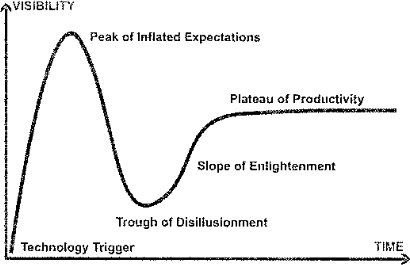
\includegraphics[width=4in]{figures/mde_pos.jpg}
\end{center}
\caption{The technology hype cycle according to \citet{brambillaBook}}
\label{mde_pos}
\end{figure}

\subsection{Model}

\begin{figure}
\begin{center}
	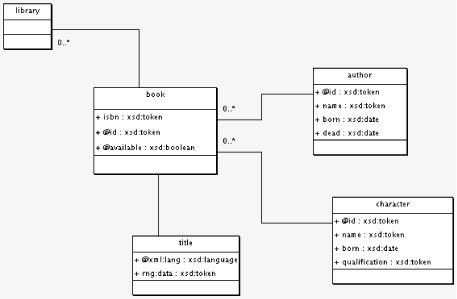
\includegraphics[width=4in]{figures/sample_model.jpg}
\end{center}
\caption{A sample model}
%TODO: Create my own model to sample here?
\label{uml_sample}
\end{figure}

A model is a representation of something that abstracts away many details that are not necessary for its use \citep{brambillaBook}. For example, the Utah Teapot \citep{utahTeapot} is a model of a teapot that is rendered by a 3D engine. However, many aspects of the teapot are not considered in its model, as they are not necessary for a simple render. An example is that the lid is not a removable component, because for the purpose of rendering the teapot, the lid never has to be removed. Another example is that the only physical property of the teapot that will be included in the model is it's finish (texture), so that lighting and reflection can be calculated. Other details such as its weight will not be included in the model, because it isnot necessary.

UML (Unified Modeling Language) is a language that is designed specifically for representing models visually. It is ideal for object-oriented design, as it represents classes with boxes and links between classes with lines. Within the boxes there are definitions of the classes (spelling?) methods and fields. In figure \ref{uml_sample}, author is a class that has properties such as name, born, dead. The diagram also shows that there is a connection between author and book.
%TODO: Write about the connection, or update to a better sample model

\subsection{Metamodels}
To have a modeling language, there must be a specification of that language that defines the valid syntax, constraints etc. In the case of UML, the Object Management Group provide a detailed specification \citep{umlSpec} of the language, and we can check that any diagram is a UML diagram by checking it against the UML specification.
%Concrete, Abstract and semantic sections...
A metamodel is the specification of a modeling language, in the form of a model \citep{brambillaBook}. A metamodel could be represented visually or textually, depending on the specification of the metamodeling language. As with many aspects of computer science, the metamodel is just another layer of abstraction, and we can continue to abstract to higher and higher levels. A metametamodel (known as M3) will define the specification of a metamodeling language, and the abstraction can continue as far as is required.

Going back to the example of The Utah Teapot, the metamodel in this case may define that the teapot is made up from interconnected polygons, and specify that each polygon has a location and size given in 3D space. 

\subsubsection{Abstract and Concrete Syntax}

When building a metamodel, both the abstract and concrete syntax must be defined. The abstract syntax of a language is a definition of how the language components interact. For an OO language, the abstract synatax would specify that a class can inherit the properties of another class, that a class must have a constructor, and that a class must be given a name. How these requirements are met by the user is specified by the concrete syntax. The concrete syntax for allowing class inheritance would state that the colon symbol must be used after the class name:

\begin{lstlisting}
class NewClass : ParentClass
\end{lstlisting}

The concrete syntax does not necessarily need to be textual. To build a modeling language you require a metamodel, which is the abstract syntax. You also require a way to visually display the model. The concrete syntax could state that a class is represented as a rectangle with the name of the class in the middle, and that to show inheritence the NewClass must have an arrow coming out of it that goes to the ParentClass that it is inheriting from.

\begin{figure}[h]
\begin{center}
	
\includegraphics[width=2in]{figures/concrete_syntax.png}
	\label{concreteSyntaxFigure}
	\caption{Concrete Syntax example for a modeling language}
\end{center}
\end{figure}

\subsection{Graphical Modeling Framework}

The Eclipse graphical modeling framework (GMF) is part of the Eclipse Graphical Modeling Project \citep{gmpSite}. The Eclipse Wiki \cite{gmpFAQ} defines GMF as:

\begin{quote} Using GMF, you can produce graphical editors for Eclipse. For example, a UML modeling tool, workflow editor, etc. Basically, a graphical editing surface for any domain model in EMF you would like. \end{quote}



\subsection{Epsilon}
To be able to perform Model Driven Engineering, we of course require some tools and languages to build and manipulate models. These tools could be built from scratch for each project, but that would be a waste of time.

Epsilon is a suite of languages and tools that provide all the necessary components to build and manipulate models. Epsilon stands for \textbf{E}xtensible \textbf{P}latform of Integrated \textbf{L}anguages for M\textbf{O}del Ma\textbf{N}agement \citep{epsilonWebsite}. It is part of the Eclipse Modeling Project \citep{ecliplseModelingProjectSite}, and includes tools for each of its languages that integrate with Eclipse. From the Epsilon Website \citep{epsilonWebsite}, the languages that are provided by Epsilon are:

\begin{description}
\item[EOL] Epsilon Object Language is an expression language that is used to create, query and model EMF models.
\item[ETL] Epsilon Transformation Language is a model-to-model transformation language.
\item[EVL] Epsilon Validation Language is a model constraint language.
\item[EGL] Epsilon Generation Language is a model-to-text generation language that can be used to generate code from models.
\item[EWL] Epsilon Wizard Language is similar to ETL, except that ETL performs batch operations whereas EWL works with in-place model transformations based on user selections.
\item[ECL] Epsilon Comparison Language is a model comparison language.
\item[EML] Epsilon Merging Language is used to merge models of diverse metamodels.
\item[Epsilon Flock] A rule
\end{description}

Together these languages provide a powerful framework for model driven engineering.

\subsection{EuGENia}
EuGENia is one of the tools that is included with Epsilon. EuGENia takes an Ecore metamodel specification and generates a GMF editor \citep{eugeniaSite}. From the code in \ref{cha:EugSampCode}, the model editor shown in figure \ref{sampleGmf} is generated by EuGENia.

\begin{figure}
\begin{center}
	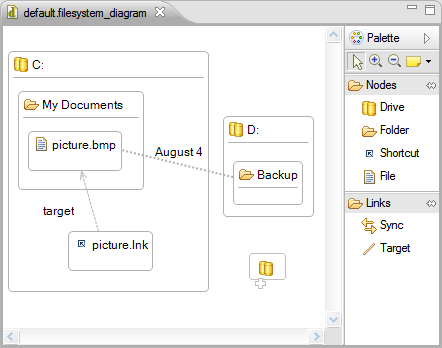
\includegraphics[width=4in]{figures/gmfeditor.png}
\end{center}
\caption{A sample gmf editor generated by EuGENia \citep{eugeniaSite}}
\label{sampleGmf}
\end{figure}

The generator editor provides the objects shown on the right hand side of figure \ref{sampleGmf}. These objects are then dragged to the left hand section of the editor by the user, where connections between objects can be intuitively created. 

\subsection{EuGENia Live}

EuGENia Live is a web-based version of EuGENia that removes some of the complexity of getting started with EuGENia. The EuGENia Live Paper \citep{eugeniaLivePaper} describes EuGENia Live as: \begin{quote}... a tool for designing graphical DSLs  \end{quote}

However, unlike EuGENia, EuGENia  Live is a visual tool that allows you to switch back and forth between graphical editing of a DSL and the code for the DSL. Figure \ref{eugeniaLiveGraphical} shows EuGENia Live graphically editing a DSL, and Figure \ref{eugeniaLiveCode} shows the same DSL's code being edited in EuGENia Live.

\begin{figure}[h]
\begin{center}
	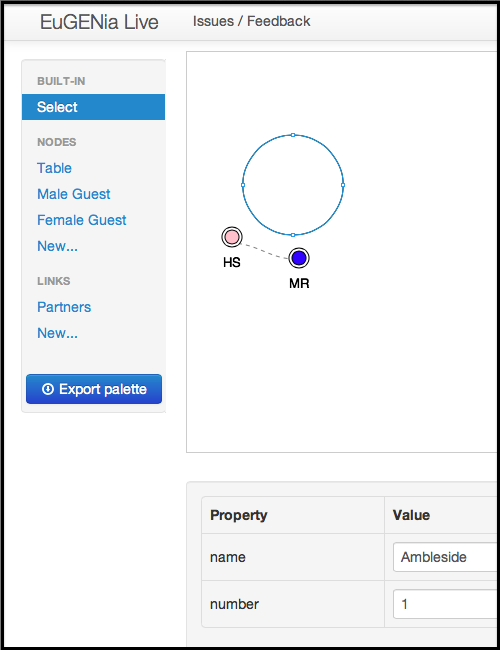
\includegraphics[width=4in]{figures/eugenia_live_graphical.png}
\end{center}
\caption{EuGENia Live's Graphical Editor \citep{eugeniaLiveDocumentation}}
\label{eugeniaLiveGraphcal}
\end{figure}

\begin{figure}[h]
\begin{center}
	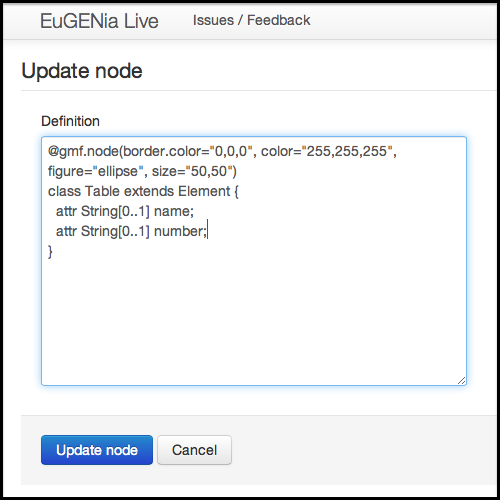
\includegraphics[width=4in]{figures/eugenia_live_code.png}
\end{center}
\caption{EuGENia Live's Code Editor \citep{eugeniaLiveDocumentation}}
\label{eugeniaLiveCode}
\end{figure}


\section{Quality of Software Testing}
\subsection{Introduction}
Software testing is a crucial part of the development cycle of any serious piece of software. Developers can make changes to code that make it do what they want, but could break another part of the program that uses the same code. Suites of tests can be implemented that \emph{should} notice if a developer breaks the code, but there is the possibility that the correct tests have not been implemented to catch a certain fault.

The Ariane 5 rocket cost \$7 billion to develop, and so of course any software on board would have had test suites to ensure that it did not fail. Unfortunately, 37 seconds after launch, \$500 million of rocket and cargo exploded because of an integer overflow \citep{ariane5}. Despite having software tests, the test `coverage' must have not been sufficient, leading to such a disaster. This is of course an extreme example, but it highlights the need for not only software testing, but good quality software testing.


% Section about testing requrements
\subsection{Coverage}

Test sets have a \emph{coverage criterion} that measures how good a collection of sets is \citep{softwareTestingIntro}. According to \citet{softwareTestingIntro}, coverage is defined as:

\begin{quote} Given a set of test requirements $TR$ for a coverage criterion $C$, a test set $T$ satisfies $C$ if and only if for every test requirement $tr$ in $TR$, at least one test $t$ in $T$ exists such that $t$ satisfies $tr$ \end{quote}

In addition to coverage, coverage level is also defined by \citep{softwareTestingIntro} as:

\begin{quote}Given a set of test requirements $TR$ and a test set $T$, the coverage level is simply the ratio of the number of test requirements satisfied by $T$ to the size of $TR$\end{quote}

\subsubsection{Code Coverage}

% ToDo: Find a source other than what Louis told me in lectures...

One approach to determining the quality of a test set is to analyse the number of lines of code that have tests that run them. If all lines of code are executed at least once when all tests have been run, then code coverage is 100\% \citep{something}. This approach is flawed however - having a line of code covered by a test does not necessarily ensure a good quality test set. Many factor can affect the result of a line of code's execution. 

Consider the code in figure \ref{sampleCoverageCode}. Even if a test covers all the lines of code in exampleProcedure, the state of globalVariable will affect the execution path and potentially the outcome of exampleFunction. This means that the tests do not cover all possible states that the program can be in.

\begin{figure}
	\begin{center}
		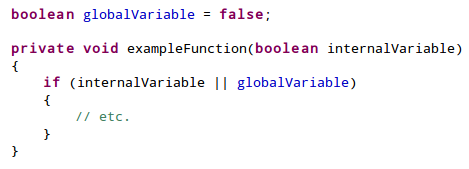
\includegraphics[width=4in]{figures/code_coverage.png}
	\end{center}
\caption{A sample code snippet}
\label{sampleCoverageCode}
\end{figure}

\subsubsection{Path Coverage}

Another approach to determining the quality of a test set is to consider the path coverage of the code being tested. A section of code can have many paths through it. In the sample code in figure \ref{sampleCoverageCode} there are two obvious paths. The first is through the if statement, the second is to skip the if statement. For a section of code with $n$ inputs, there are potentially $2^n$ code paths \cite{something}. This can of course be problematic, because for any program larger than a few lines of code the numbers of code paths will be very large, quickly getting to the point where it is not feasible to compute all paths, and therefore not possible to check if all paths are covered by a test set.

\subsection{Mutation Testing}

Mutation testing is another approach to determining the quality of a test set. Consider the following line of code:

\begin{lstlisting}
y := 3x + 4 - z;
\end{lstlisting}

This is the fragment of code that we want to check that our test sets sufficiently cover. The code is called the \emph{ground string}. From the ground string, mutant strings are created. These mutant strings are based on the ground string, but have been `mutated' in some way such that they are not the same as the ground string, but still compile \citep{softwareTestingIntro}. Some example mutants might be:

\begin{lstlisting}
y := 3x - 4 - z;
y := 3x - 4 + z;
y := 10x + 6 - i;
\end{lstlisting}

The mutants all compile, but alter the outcome of executing the function. So the quality of a test set can be determined by running the set on each of the mutants and checking how many of the mutants are rejected. The perfect test set would reject all of the mutants \citep{softwareTestingIntro}. The example above is greatly simplified, and in reality it is unlikely that all of the mutants would be caught by the test set.

In addition to being used to determine the quality of test sets, mutation testing (and path coverage and code coverage) can be used to help develop a high quality test set \citep{softwareTestingIntro}.

\subsection{Model Transformation Testing}

EuGENia is a model transformation written in ETL. It takes an Ecore metamodel as an input and generates gmf models as an output\citep{eugeniaSite}. One approach to verifying and possibly improving the consistency between EuGENia and EuGENia Live is to ensure that both applications have a good quality test suite.

\citet{mttBarriers} describe the three stages to model transformation testing:

\begin{enumerate}
	\item Generate test data: As with any type of test, there needs to be some input to the system. In this case it will be a set of models that are to be transformed. These models will conform to the metamodel that specifies input to the model transformation, and will either be manually created by the tester, or automatically generated in the form of graphs of metamodel instances \citep{mttBarriers}.
	\item Define test adequacy criteria: For any modeling language beyond the very basic there will be a very large number of possible inputs. This rules out running every possible model through the transformer in to test it as it would take too long. Instead a test adequacy criteria must be defined that allows the effective seletion of test models. According to \citet{mttBarriers}, there is no well-defined criteria for model transformation testing.
	\item Construct an oracle: The oracle gets the output of the system and determines if it is correct (based on the test input model).
\end{enumerate}

%ToDo: Write about quality of model testing here

The oracle can be difficult to create for any complex model transformation. \citet{mttOracleIssue} propose six ways that an oracle could be implemented for model transformation testing:

\begin{enumerate}
	\item Compare the output to a reference model (i.e. the expected output model for the particular input). Unfortunately this requires that the tester has to create the expected models for each test. For a large test set this could be incredibly time consuming.
	\item Perform an inverse transformation on the output. This would give the original input model, if the model transformation was correct. This requires that the tester implement a reverse transformation, and also requires that the transformation is an injective function (i.e. a function that preserves distinctness). According to \citet{mttOracleIssue}, this is unfortunately unlikely.
	\item Compare the output with that from a reference model transformation. This reference model transformation can produce the reference model from the test model. 
	\item A generic contract is a list of constraints on the output of the model transformation based on the input. Once the model transformation has completed the output model is checked against the constraints defined in the generic contract.
	\item The tester could provide a list of assertions in OCL (or EVL) that can be checked on the output model. Not every detail about the output model must be provided. Doing so would be a waste of time as providing the expected output model would be quicker.
	\item Model snippets could be provided by the tester. Each snippet is associated with a cardinality and logical operator so that the expected number of occurrences of each snippet can be calculated. The oracle would check that the expected number of each snippet appears in the output. 
\end{enumerate}




% Close chapter with testing of model transformations
% Barriers to systematic model transformation testing 2010
% Qualifying input test data for model transformations
% Model transformation testing : Oracle Issue

% 
